\chapter{Introduzione}
\textbf{L'Arcobaleno della Cittadinanza Digitale} è un \emph{framework} il cui scopo è quello di rappresentare gli aspetti della cittadinanza digitale in livelli concettuali. Il modello è così articolato:
\begin{itemize}
    \item I livelli più bassi definiscono le caratteristiche tecnico-infrastrutturali,
    \item I livelli più alti riguardano il diritto di un cittadino al coinvolgimento attivo nel processo decisionale.
\end{itemize}
\begin{figure}[h!]
    \centering
    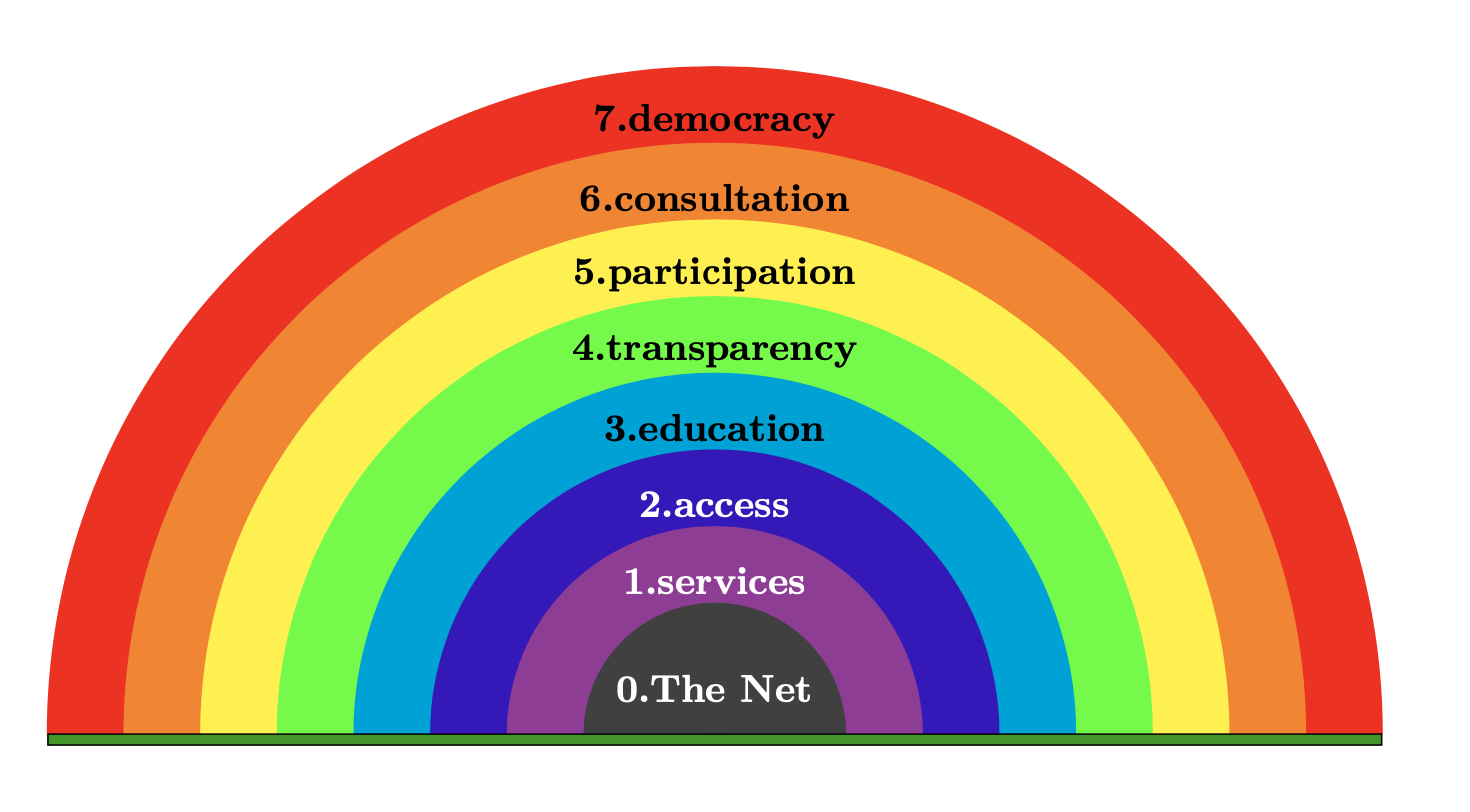
\includegraphics[scale=0.5]{img/rainbow.png}
    \caption{Arcobaleno della Cittadinanza Digitale e Tecnocivismo}
    \label{fig:rainbow}
\end{figure}
